\section{Introduction}

In this section we will tour some phenomena concerning the loci of triangle centers over elliptic billard 3-periodics, including the loci of vertices of certain derived triangles.

Recall the loci of the incenter $X_1$ and excenters (vertices of the excentral family) were previously shown to be ellipses, see \cref{sec:03-inc-exc-loci} and \cref{fig:billiard-grid}. Recall also that the locus of the Mittenpunkt $X_9$ is a point, see \cref{sec:03-stationary}.

\begin{itemize}
\item confocal
    \begin{itemize}
        \item loci of incenter, excenters
        \item loci of intouchpoints
        \item loci od X1,X2,X3,X4,X5
        \item loci of X11 and X100
        \item loci of derived triangle vertices: extouch (caustic), intouch (sextic), feuerbach triangle, medial, anticomplementary 
    \end{itemize}
    \item brocard points
\end{itemize}

We will omit most proofs etc.

\section{Loci of the first five Kimberling centers}

The semi-axes $a_1,b_1$ for the elliptic locus of the incenter $X_1$ were given in \cref{thm:03-incenter-excenter}. It turns the loci of the next four centers in \cite{etc} are also ellipses. There are the barycenter $X_2$, the circumcenter $X_3$, the orthocenter $X_4$, and the center of the 9-point circle (also known as Euler's circle) $X_5$. Their semi-axes are given by:

\begin{align*}
    \left(a_2,b_2\right)=&k_2\left(a,b\right),\;\text{with}\; k_2=\frac{2\delta -a^{2}-b^{2}}{3c^2}\\
     \left(a_3,b_3\right)=&\left(\frac{a^{2}-\delta}{2a},\frac{\delta-b^{2}}{2b}\right)\\
 \left(a_4,b_4\right)=&\left(\frac{k_4}a,\frac{k_4}b\right),\;\text{with}\;k_4=\frac{  (a^{2}+b^{2})\delta-2\,a^{2}b^{2} }{c^2}\\
   \left(a_5,b_5\right)=&\left(\frac{- w'_5(a,b)+ w''_5(a,b) \delta}{ w_5(a,b)},\;\frac{ w'_5(b,a)-{w''_5(b,a) \delta}}{w_5(b,a)}\right)
\end{align*}
where $w'_5(u,v)=u^2(u^2+3v^2)$, $w''_5(u,v)=3u^2+ v^2$, and $w_5(u,v)=4u(u^2-v^2)$. Note that (i) $a_2/b_2=a/b$ and (ii) $b_4/a_4=a/b$.

As it turns out, the locus of 49 out of the first 200 centers in \cite{etc} are ellipses. These are: $X_k$, $k=$1,  2,  3,  4,  5,  7,  8,  10,  11,  12,  20,  21,  35,  36,  40,  46,  55,  56,  57,  63,  65,  72,  78,  79,  80,  84,  88,  90,  100,  104,  119,  140,  142,  144,  145,  149,  153,  162,  165,  190,  191,  200. Links to live animations as well as expressions for their semi-axes are provided in \cite{garcia2021-ellipses-web}.

%% Swans
%% the following centers lie on the $X_9$-centered circumellipse: 88, 100, 162, 190 \cite{etc}.

\begin{figure}
\centering
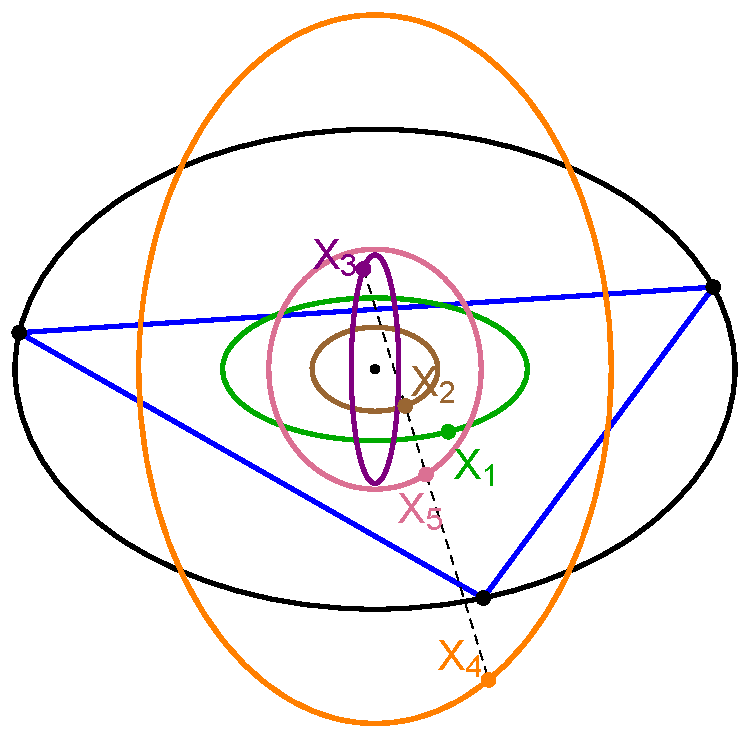
\includegraphics[width=.6\textwidth]{pics_04_060_locus_x12345.pdf}
\caption{Over billiard 3-periodics, the loci of incenter $X_1$, barycenter $X_2$, circumcenter $X_3$, orthocenter $X_4$, and 9-point center $X_5$ are all ellipses. The Euler line (dashed black) is shown passing through all but the first center. \href{https://youtu.be/sMcNzcYaqtg}{Video}, \href{https://bit.ly/3eVScgE}{Live}}
\label{fig:04-x12345}
\end{figure}

%%% begin X4
\section{When billiard 3-periodics are obtuse}

\begin{figure}
    \centering
    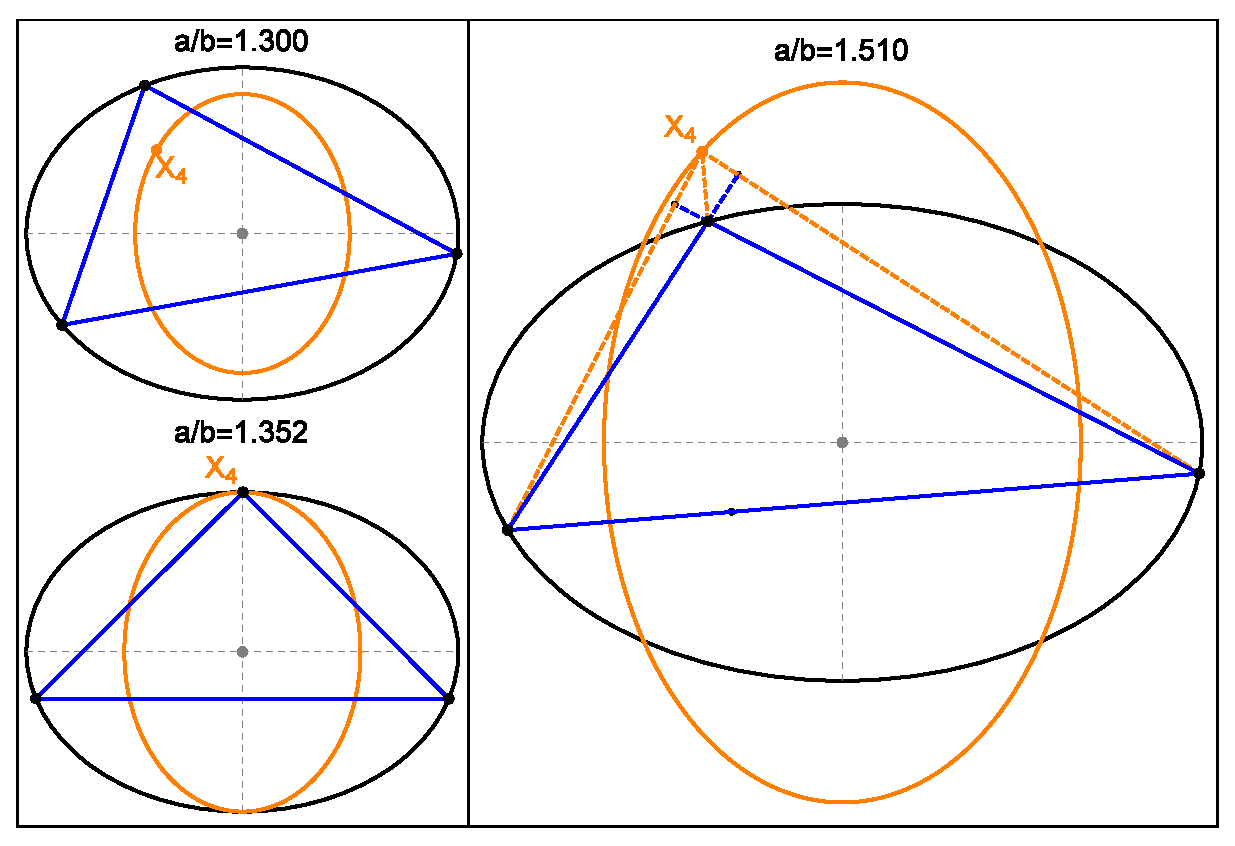
\includegraphics[width=\textwidth]{pics_04_130_ort_loci.eps}
    \caption{Locus of the orthocenter (orange) over elliptic billiards with different aspect ratios. If $a/b$ is (i) less than (resp. (ii) equal, (iii) greater than) $\alpha_4{\simeq}1.352$, the locus of the orthocenter $X_4$ (orange) is (i) interior (resp. (ii) internally tangent, (iii) intersecting) with the elliptic billiard. In (i) and (ii) all 3-periodics are acute, whereas in (iii) some will be obtuse.}.
    \label{fig:04-orthocenter-loci}
\end{figure}

It turns out the locus of $X_4$ can be used to determine if the billiard 3-period family will contain obtuse triangles. Referring to Figure~\ref{fig:04-orthocenter-loci}:

\begin{proposition}
The locus of $X_4$ is internally tangent to the elliptic billiard at its top and bottom vertices when $a/b=\alpha_4$ given by:

\[\alpha_4 = \sqrt{2\,\sqrt {2}-1}\;{\simeq}\;1.352.\]
\label{prop:04-alpha4}
\end{proposition}

\begin{proof}
The equation $b_4=b$ is equivalent to $a^4+2a^2b^2-7b^4=0.$ Therefore, as $a>b>0$, it follows that $a/b=\sqrt{2\,\sqrt {2}-1}.$
\end{proof}

\noindent Let $\alpha_4^*$ be the positive root of
${x}^{6}+{x}^{4}-4\,{x}^{3}-{x}^{2}-1=0$, i.e.,
$\alpha_4^{*}={\simeq}\;1.51$. 

\begin{proposition}
When $a/b=\alpha_4^{*}$, then $a_4=b$ and $b_4=a$, i.e., the locus of $X_4$ is identical to a rotated copy of Billiard. 
\end{proposition}

\begin{proof}
The condition $a_4=b$, or equivalently $b_4=a$, is defined by $a^6+a^4b^2-4a^3b^3-a^2b^4-b^6=0$. Graphic analysis shows that ${x}^{6}+{x}^{4}-4\,{x}^{3}-{x}^{2}-1=0$ has only one positive real root which we call $\alpha_4^*$.
\end{proof}

\begin{theorem}
If $a/b<\alpha_4$ (resp. $a/b>\alpha_4$) the 3-periodic family will not (resp. will) contain obtuse triangles.
\end{theorem}

\begin{proof}
If the 3-periodic is acute, $X_4$ is in its interior, therefore also internal to the EB. If the 3-periodic is a right triangle, $X_4$ lies on the right-angle vertex and is therefore on the EB. If the 3-periodic is obtuse, $X_4$ lies on exterior wedge between sides incident on the obtuse vertex (feet of altitudes are exterior). Since the latter is on the EB, $X_4$ is exterior to the EB.
\end{proof}

Another way to think of this is depicted in \cref{fig:04-obtuse-zones}: $a/b>\alpha_4$, opens up two ``zones'' along the top and bottom halves of the elliptic billiard. A 3-periodic will be obtuse if and only if one of its vertices is on either zone. These zones are precisely portions of the elliptic billiard which are interior to the locus of $X_4$; see \cref{fig:04-orthocenter-loci}(right). When $a/b=\alpha_4$ said zones collapse to the top and bottom vertices of the elliptic billiard; see \cref{fig:04-orthocenter-loci}(bottom left).

\begin{figure}
    \centering
    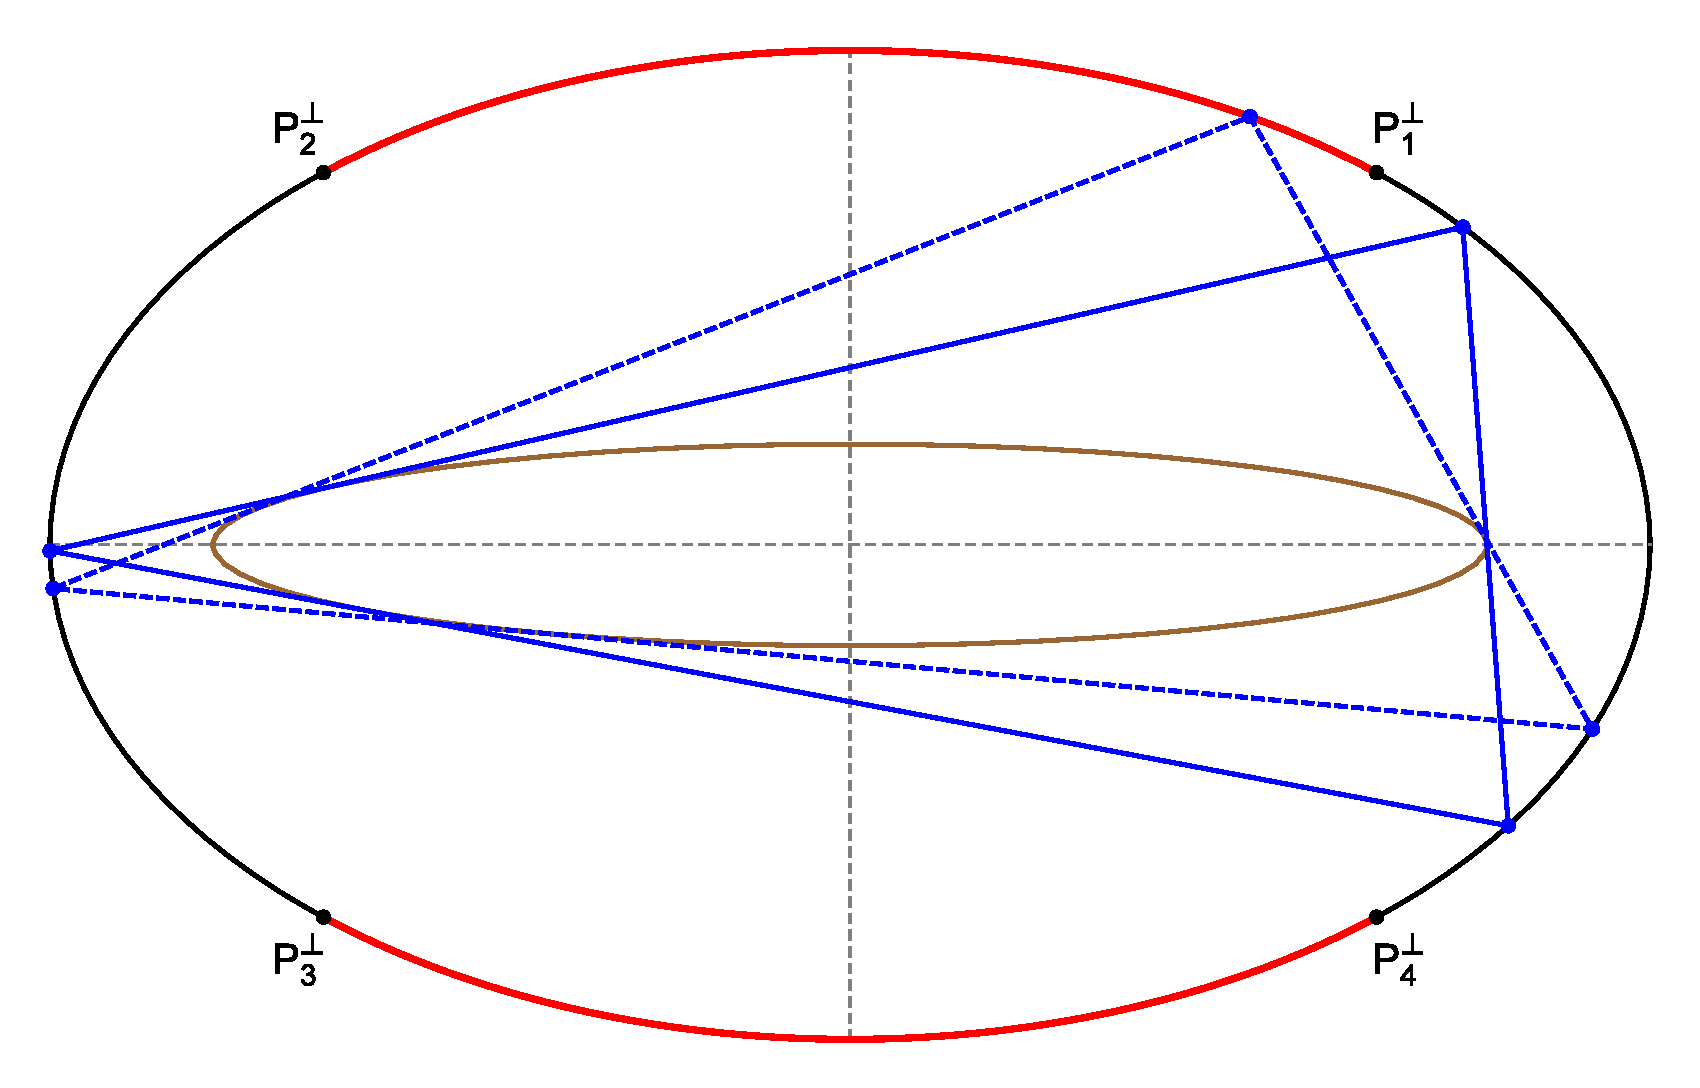
\includegraphics[width=.66\textwidth]{pics_04_150_rect_zones.eps}
    \caption{Both acute (blue) and obtuse (dashed blue) billiard 3-periodics are shown. In this case $a/b=1.618>\alpha_4$. If a 3-periodic vertex is located in the red arcs along the top and bottom halves of the elliptic billiard, the 3-periodic will be obtuse.}
\label{fig:04-obtuse-zones}
\end{figure}

%%% end X4

%%% begin X6
\section{Quartic locus of the symmedian point \torp{$X_6$}{X(6)}}
\label{sec:symmedian}

The symmedian point $X_6$ is replete with properties, indeed it is known as the crown jewel of triangle geometry \cite[Symmedian Point]{mw}. Its construction is deceptively simple: the point where a triangle's {\em symmedians} concur; these are reflections of medians on the bisectors. Its trilinear coordinates could not be simpler: $[a:b:c]$. However, it is the first Kimberling center whose locus over billiard 3-periodics is {\em not} an ellipse. 

In fact, when $1<a/b<2$, its locus is visually indistinguishable from a true ellipse; see Figure~\ref{fig:04-locus-x6}. Fortunately, its fit error is easily detectable with numerical methods. Indeed:

\begin{proposition}
The locus of $X_6$ is a convex quartic given by:

\begin{equation*}
  \X_6(x,y)=c_1 x^4+c_2 y^4+c_3 x^2 y^2+ c_4 x^2 + c_5 y^2 = 0
\end{equation*}

\noindent where:
$$
\begin{array}{rlrl}
c_1=&b^4(5\delta^2-4(a^2-b^2)\delta -a^2 b^2)&c_2=&a^4(5\delta^2+4(a^2-b^2)\delta-a^2b^2) \\
c_3=&2a^2 b^2(a^2 b^2+3\delta^2)&c_4=&a^2 b^4(3 b^4+2(2 a^2-b^2)\delta-5\delta^2)\\
c_5=&a^4 b^2(3 a^4+2(2 b^2-a^2)\delta-5\delta^2)&\delta=&\sqrt{a^4-a^2 b^2+b^4}
\end{array}
$$
\end{proposition}

\begin{proof}
Using a CAS, obtain symbolic expressions for the coefficients of a quartic symmetric about both axes (no odd-degree terms), passing through 5 known-points. Still using a CAS, verify the symbolic parametric for the locus satisfies the quartic.
\end{proof}

 \noindent Note the above is also satisfied by a degenerate level curve $(x,y)=(0,0)$, which we ignore.

\begin{remark}
We term the ``best-fit'' ellipse $\mathcal{E}_6$ the one internally-tangent to $\X_6(x,y)=0$ at its four vertices. Its semi-axes are given by: 

{\small  
\begin{align*}
%a_6=&\frac{\left[(3\,a^2-b^2)\delta %-(a^2+b^2)b^2\right]a}{a^4+b^4+2\delta^2}\nonumber\\
a_6= \frac{\left[(3\,a^2-b^2)\delta -(a^2+b^2)b^2\right]a}{a^2b^2+3\delta^2},\;\;\;
b_6= \frac{\left[(a^2-3\,b^2)\delta + (a^2+b^2)a^2\right]b}{a^2b^2+3\delta^2}
\label{eqn:x6-ellipse}
\end{align*}
}
\end{remark}

Table~\ref{tab:quartic-coeffs} shows the above coefficients numerically for a few values of $a/b$.

\begin{table}
    \centering
$$
\begin{array}{|c|c|c|c|c|c|c|c|}
\hline
 \text{a/b} & a_6 & b_6 & c_1/c_3 & c_2/c_3 & c_4/c_3 & c_5/c_3 & A(\mathcal{E}_6)/A(\mathcal{X}_6) \\
 \hline
  1.25 & 0.433 & 0.282 & 0.211 & 1.185 & -0.040 & -0.095 & 0.9999 \\
 1.50 & 0.874 & 0.427 & 0.114 & 2.184 & -0.087 & -0.399 & 0.9998 \\
 2.00 & 1.612 & 0.549 & 0.052 & 4.850 & -0.134 & -1.461 & 0.9983 \\
 3.00 & 2.791 & 0.620 & 0.020 & 12.423 & -0.157 & -4.769 & 0.9949 \\
 \hline
\end{array}
$$
\caption{Coefficients $c_i/c_3$, $i=1,2,4,5$ for the quartic locus of $X_6$ as well as the axes $a_6,b_6$ for the best-fit ellipse, for various values of $a/b$. The last-column reports the area ratio of the internal ellipse $\mathcal{E}_6$ (with axes $a_6,b_6$) to that of the quartic locus $\mathcal{X}_6$, showing an almost exact match.}
\label{tab:quartic-coeffs}
\end{table}


\begin{figure}
    \centering
    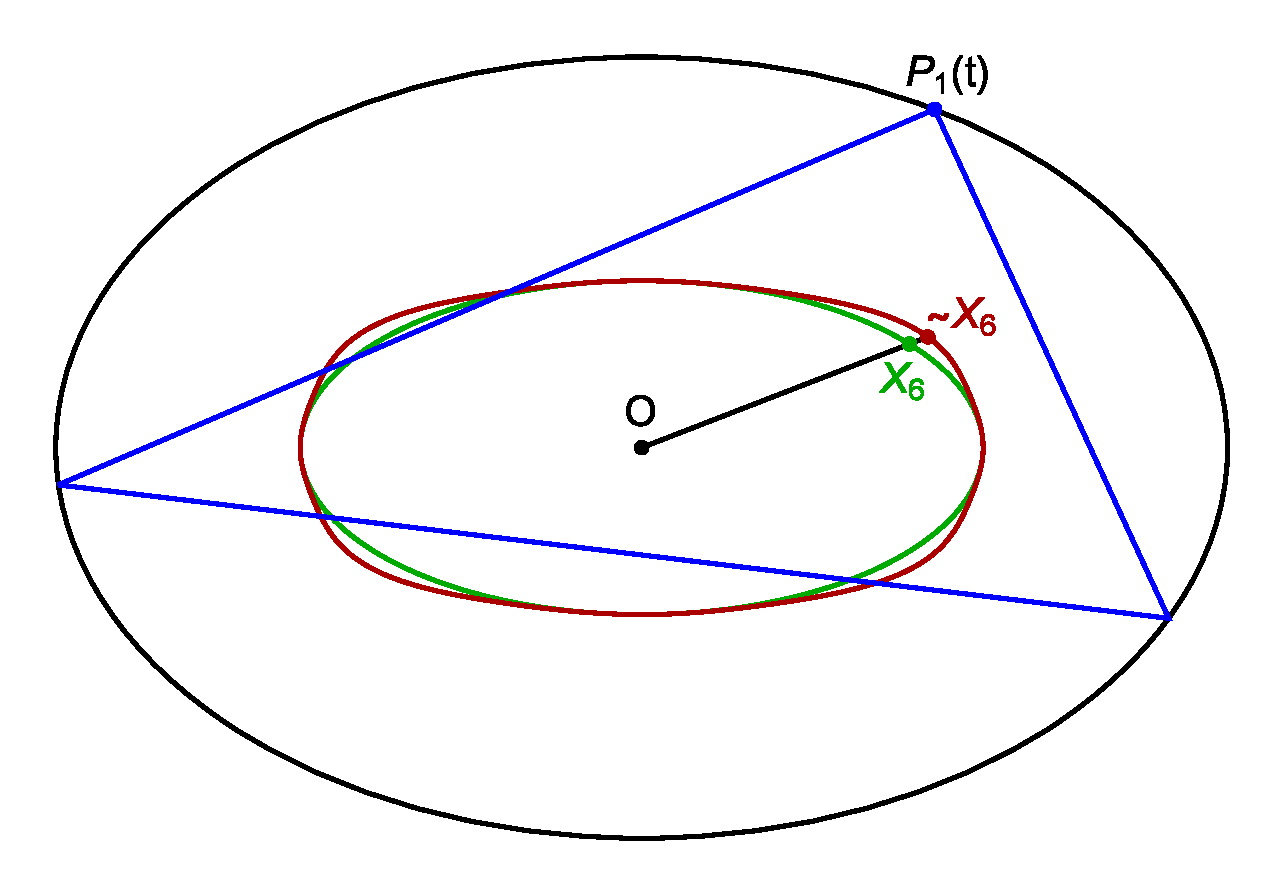
\includegraphics[width=.7\textwidth]{pics_04_090_symmedian.eps}
    \caption{Over billiard 3-periodics (blue), the locus of the symmedian point $X_6$ is a quartic (green). At the billiard aspect ratio shown, it is visually identical to an ellipse. Also shown is a copy of the quartic (red) such that the distance to a best-fit ellipse (green) is scaled 1000 fold. \href{https://bit.ly/3hxOZoV}{Live}}
    \label{fig:04-locus-x6}
\end{figure}
%%% end X6

%%% BEGIN X11 and X100
\begin{figure}
    \centering
    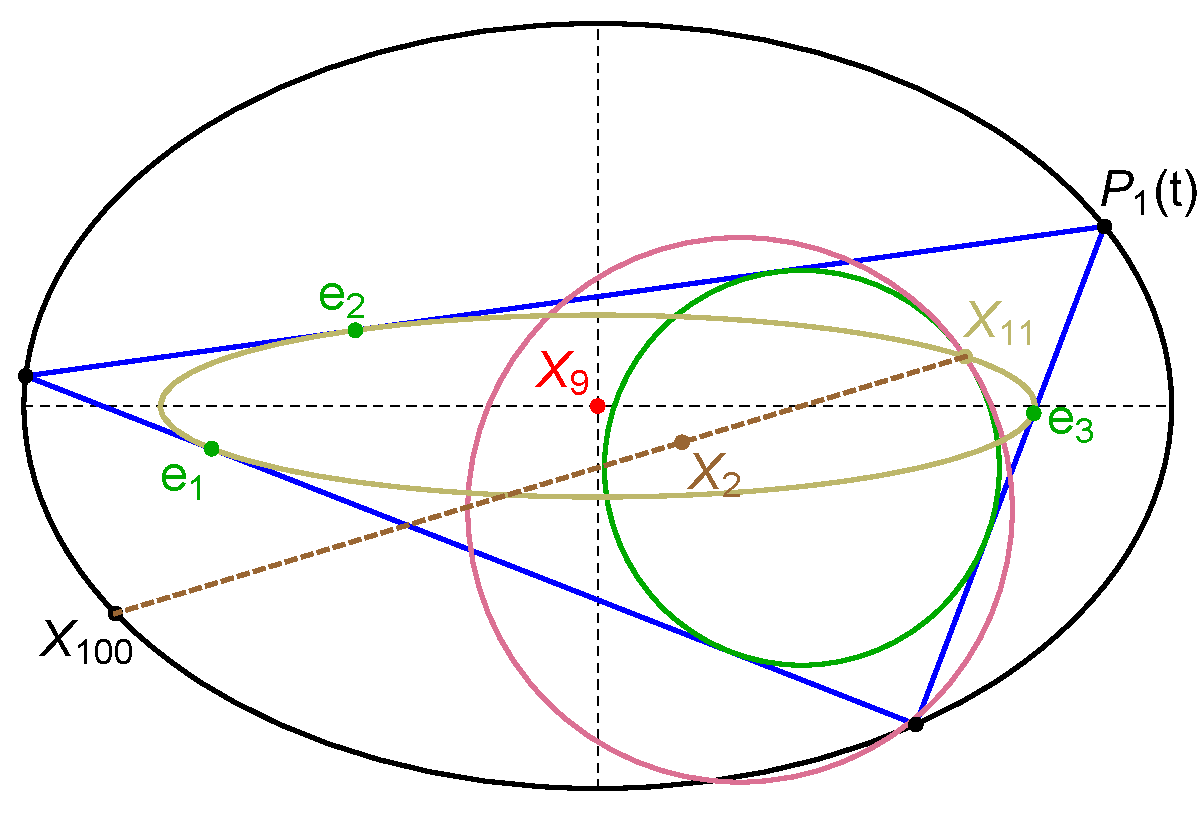
\includegraphics[width=.7\textwidth]{pics_04_080_feuerbach_loci.pdf}
    \caption{A billiard 3-periodic (blue). Also shown are the incircle (green) and 9-point circle (pink) which touch at the Feuerbach point $X_{11}$. Also shown is the latter's {\em anticomplement} $X_{100}$, and the three extouchpoints $e_1,e_2,e_3$. Over the billiard family, $X_{100}$ sweep the billiard while both $X_{11}$ and the extouchpoints sweep the caustic (though in opposite directions).
    % done
    \href{https://youtu.be/TXdg7tUl8lc}{Video},
    \label{fig:04-feuer-loci} \href{https://bit.ly/2S2LVqp}{Live}}
\end{figure}

\section{The locus of the Feuerbach point and its anticomplement}

Referring to \cref{fig:04-locus-x11-x100}, the Feuerbach point $X_{11}$ is the single point of contact between incircle and 9-point circle \cite[X(11)]{mw}. $X_{11}$ is known to lie on the $X_{9}$-centered inconic, i.e., the  Mandart inellipse \cite[Mandart inellipse]{mw}. Since the latter is unique:

\begin{observation}
The confocal caustic is the stationary Mandart inellipse of billiard 3-periodics.
\end{observation}

Therefore:

\begin{proposition}
Over billiard 3-periodics, $X_{11}$ sweepts the confocal caustic.
\end{proposition}

The anticomplement of a point $P$ is its double-length reflection about the barycenter $X_2$, i.e., $A(P) = X_2+2 X_2-P$. Stille referring,  \cref{fig:04-locus-x11-x100}, $X_{100}$ is the anticomplement of $X_{11}$. This point is known to lie on (i) the circumcircle, (ii) the Steiner circumellipse (centered on $X_2$), and most relevantly here, (iii) on the $X_9$-centered circumellipse \cite[X(9)]{etc}. Since the latter is unique:

\begin{observation}
The elliptic billiard is the stationary $X_9$-centered circumconic of billiard 3-periodics.
\end{observation}

Therefore:

\begin{proposition}
Over billiard 3-periodics, the locus of $X_{100}$ is the elliptic billiard.
\end{proposition}

The vertices of the so-called {\em extouch triangle} are the points of contact of the excircles with a triangle's sidelines \cite[Extouch triangle]{mw}. These are also known as {\em extouchpoints}. A known fact is that the Mandart inellipse (i.e., the caustic) touches a triangle's sidelines at the extouchpoints \cite[Mandart inellipse]{mw}. Therefore:

\begin{proposition}
Over billiard 3-periodics, the locus of the extouchpoints is the confocal caustic.
\end{proposition}

This is also illustrated in \cref{fig:04-locus-x11-x100}. A curious dynamic phenomenon is that while the extouchpoints follow the direction of motion of billiard 3-periodics along the outer ellipse (e.g., counter- or clockwise), $X_{11}$ rotates in the opposite direction; see this \href{https://bit.ly/2S2LVqp}{Live}.


%%% END X11 and X100

\section{Locus of vertices of some derived triangles}

A few triangles derived from billiard 3-periodics are shown in \cref{fig:04-derived-isosceles}. For their definitions see \cite{app:app-triangle} and \cite{mw}.

\begin{figure}
    \centering
    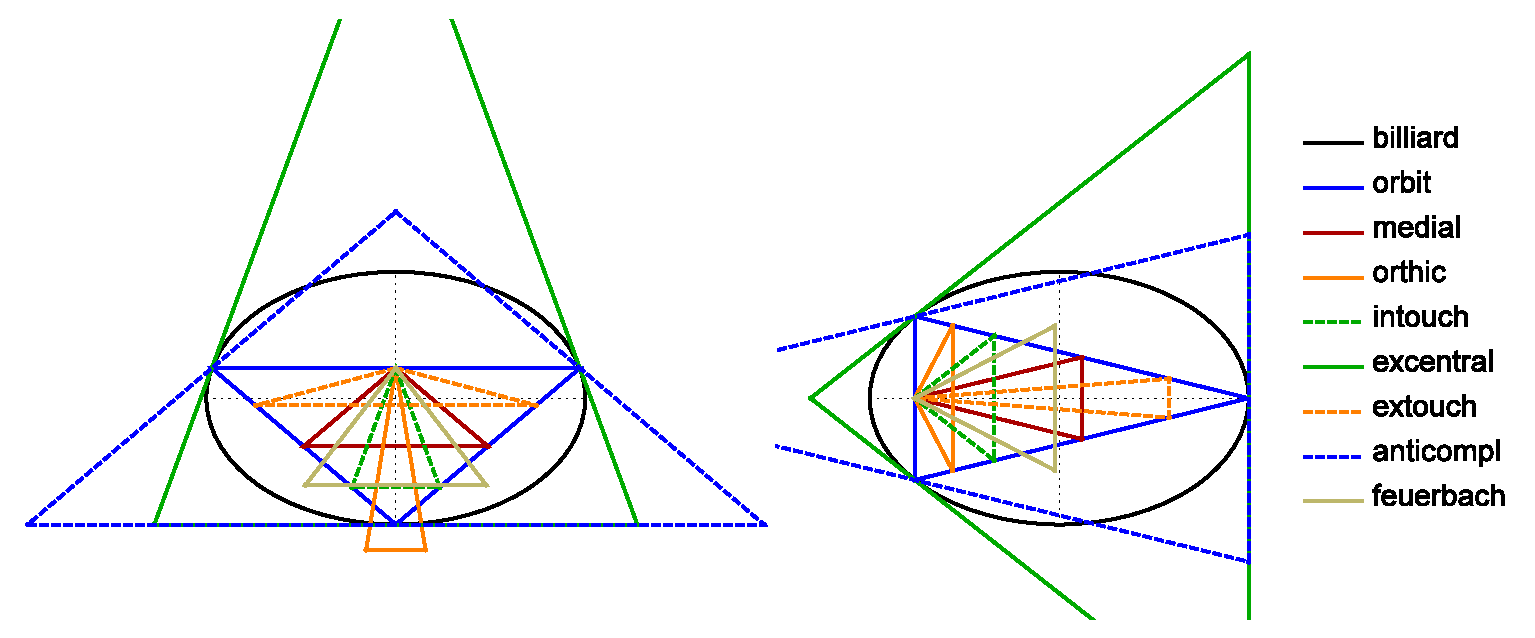
\includegraphics[width=\textwidth]{pics_04_100_confocal_derived.eps}
    \caption{Triangles derived from an isosceles billiard 3-periodic (blue). These contain one vertex on the axis of symmetry. \href{https://youtu.be/xyroRTEVNDc}{Video}, \href{https://bit.ly/3fyylD0}{Live}}
    \label{fig:04-derived-isosceles}
\end{figure}

Mentioned in \cref{sec:01-introduction} was an early experiment which showed that over billiard 3-periodics, the locus of the vertices of the intouch triangle (i.e., the intouchpoints) is a 2-lobed, self-intersect curve; see \cref{fig:01-intouch-x59}.

As shown in \cref{fig:04-locus-x11-x100}, the loci of vertices of some other triangles derived from billiard 3-periodics aren't ellipses. A noteworthy exception is the extouch triangle, mentioned above.

\begin{figure}
    \centering
    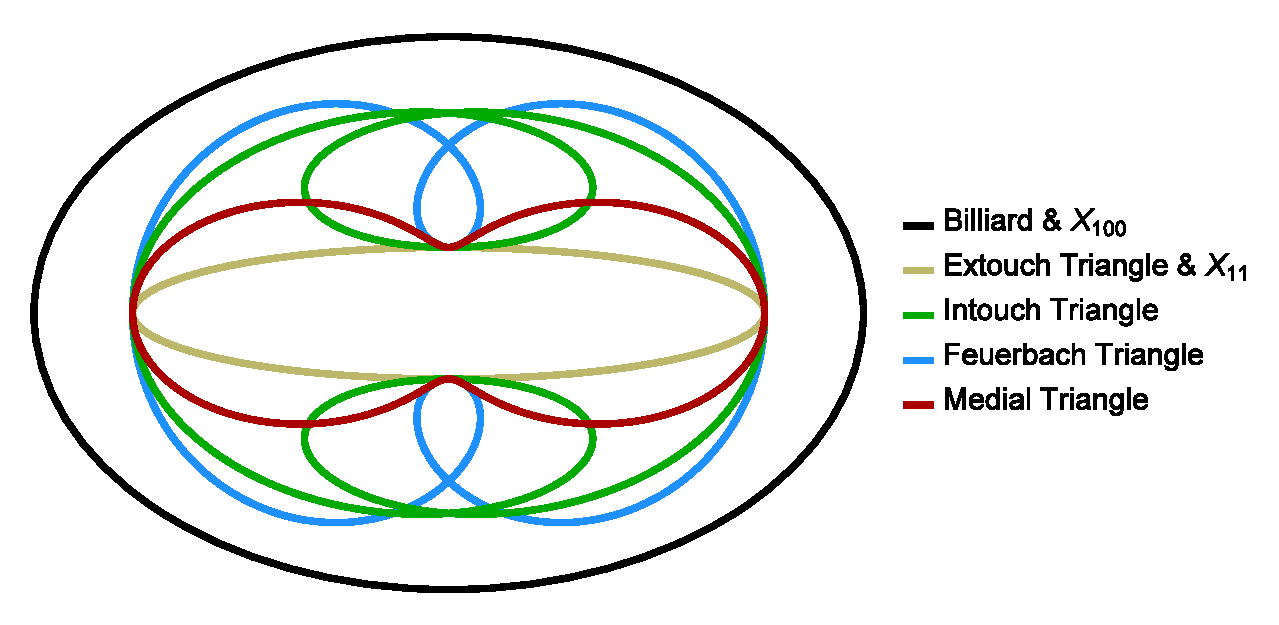
\includegraphics[width=\textwidth]{pics_04_070_non_elliptic.eps}
    \caption{Non-elliptic loci of the vertices of triangles derived from billiard 3-periodics: the (i) intouch (green), (ii) Feuerbach (not to be confused with the Feuerbach {\em point}) (blue), (iii) medial (red), triangles. A noteworthy excpetion is the extouch triangle (light brown), whose vertices sweep the confocal caustic.
     \href{https://youtu.be/OGvCQbYqJyI}{Video}, \href{https://bit.ly/3orrSxQ}{Live}}
    \label{fig:04-locus-x11-x100}
\end{figure}

\section{Orthic incenter: a locus with kinks}

Loci considered thus far have been smooth, regular curves. Here we give an example of one with four corners. Recall that given a triangle $T$, the orthic triangle has vertices at the feet of $T$'s altitudes.

\begin{figure}
    \centering
    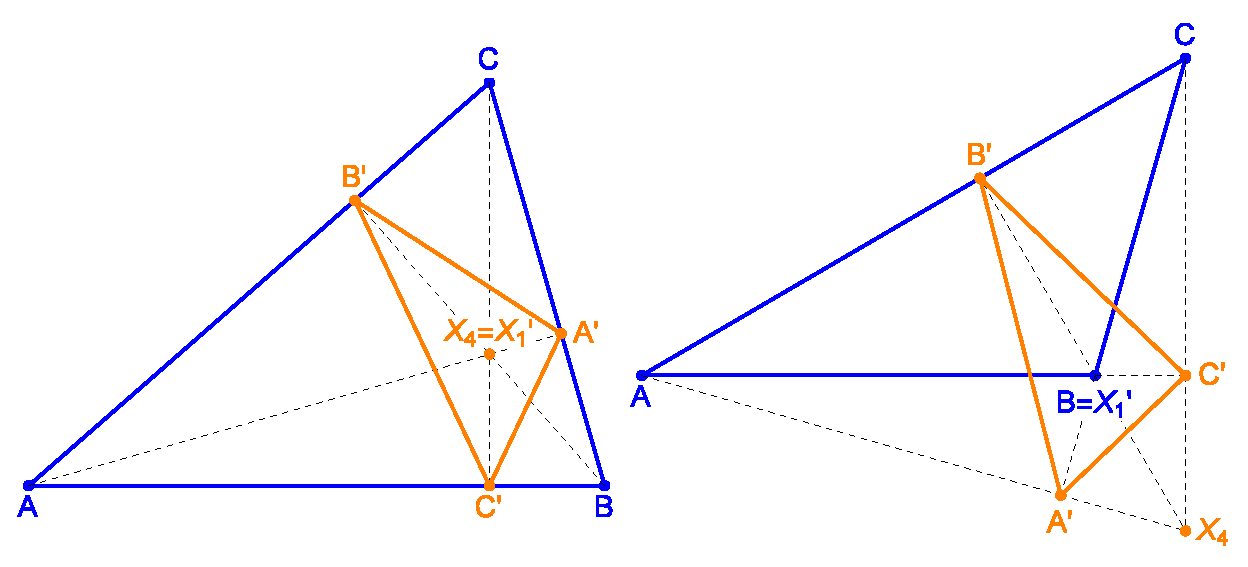
\includegraphics[width=.8\textwidth]{pics_04_140_orthic_incenter.eps}
    \caption{\textbf{Left}: the orthic triangle (orange) is shown of an acute reference triangle $T$ (blue), for with an interior orthocenter $X_4$. In this case, the orthic incenter $X_1'$ coincides with $X_4$. \textbf{Right}: When $T$ (blue) is obtuse, $X_4$ is exterior. Furthermore, two orthic vertices are outside of $T$ and $X_1'$ coincides with the obtuse vertex, $B$ in the picture. \href{https://youtu.be/-bLuvICzmqM}{Video}}
    \label{fig:04-orthic-incenter}
\end{figure}

Referring to \cref{fig:04-orthic-incenter}, 
it is easy to see that if a triangle $T$ is acute (resp. obtuse), all three vertices (only one vertex) of the orthic will lie on a sideline. In the obtuse case, the other two will lie on extensions of two sidelines, i.e., they will be exterior to $T$.

An interesting result, mentioned in \cite[Chapter 1]{coxeter67}, is the ``switching'' behavior of the incenter of the orthic triangle:

\begin{lemma}
If a triangle is acute (resp. obtuse), the incenter of the orthic will coincide with the orthocenter (resp. the obtuse vertex of $T$).
\label{lem:04-pinned}
\end{lemma}

Recall that for billiard 3-periodics to include obtuse triangles, $a/b>\alpha_4$; see \cref{prop:04-alpha4}. Referring to
\cref{fig:04-orthocenter-loci}:

% \includegraphics[trim={left bot right upper},clip]
\begin{figure}
    \centering
    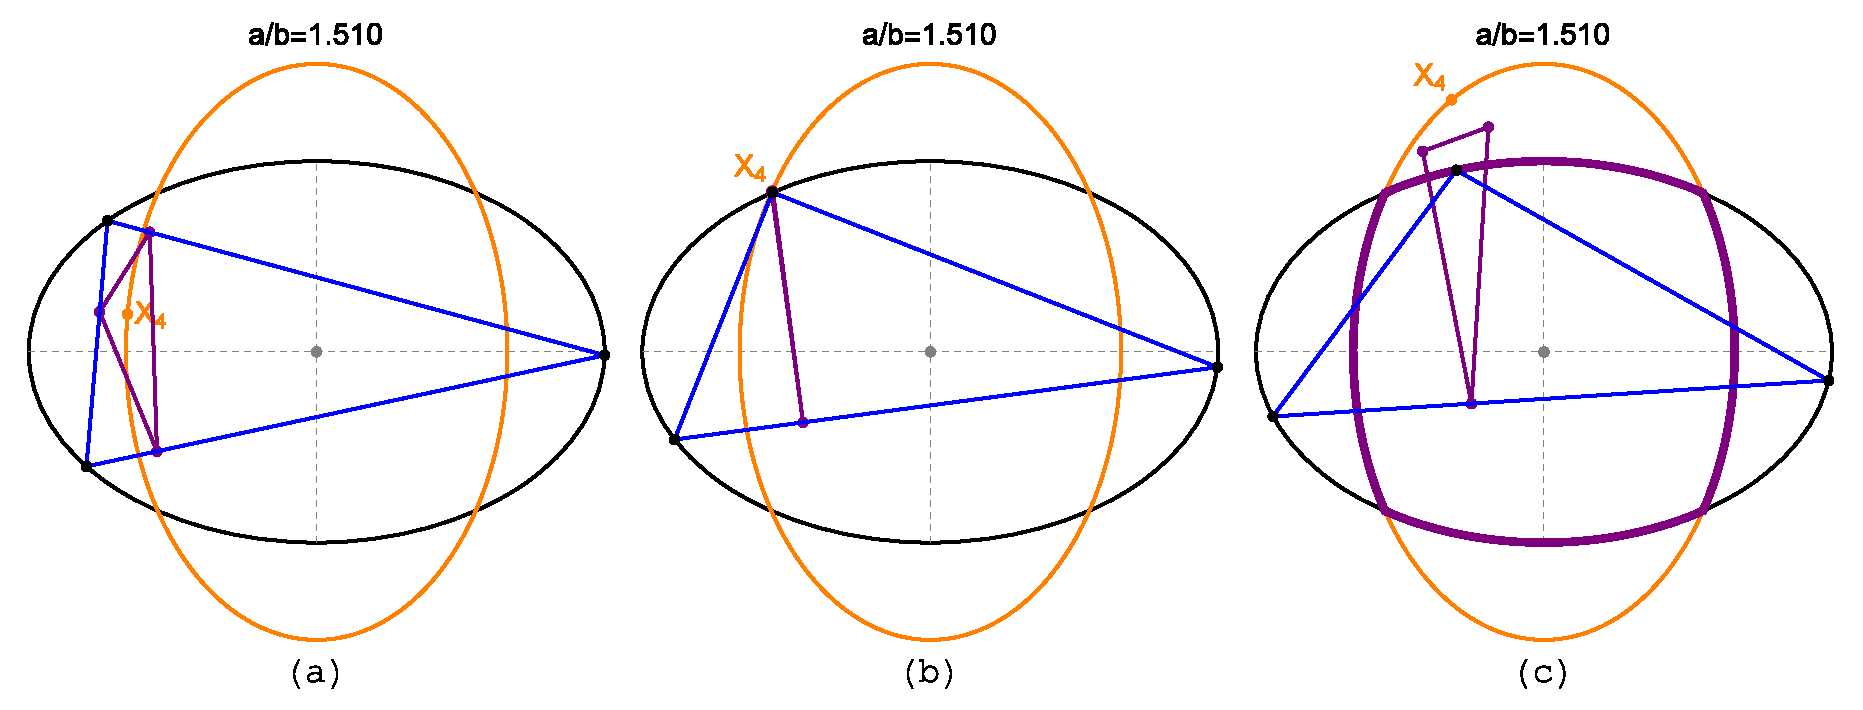
\includegraphics[trim={0 0 0 20},clip,width=\textwidth]{pics_04_120_ort_loci_kink.eps}
    \caption{From left to right: the orthic triangle (purple) of billiard 3-periodics (blue) is shown at 3 different positions. The locus of $X_4$ (orange ellipse) intersects the billiard, i.e., $a/b>\alpha_4$. When a 3-periodic is acute (left), the orthic incenter coincides with $X_4$. When it is a right triangle (middle), $X_4$ is on the elliptic billiard and the orthic is a degenerate segment. When it is obtuse (right), the orthic incenter remains ``pinned'' to the obtuse vertex. The end result is that the locus of the orthic incenter is a quadrilateral with four elliptic arcs (thick purple, right) with four corners.  \href{https://youtu.be/3qJnwpFkUFQ}{Video}, \href{https://bit.ly/33TVjit}{Live}}
    \label{fig:04-orthic_incenter_locus}
\end{figure}

\begin{corollary}
If $a/b>\alpha_4$, the locus of the incenter of the orthic triangle of billiard 3-periodics is an elliptic arc ``quadrilateral'' with four corners.
\end{corollary}

%%% begin self-inter

\section{The self-intersecting locus of \torp{$X_{59}$}{X(59)}}

Consider the curious case of a triangle center which is the isogonal conjugate of the Feuerbach point, listed on \cite{etc} as $X_{59}$. We revisit its intriguing locus, shown previously in \cref{fig:01-intouch-x59}(right).

This is a continuous curve with four self-intersections, internally tangent to the elliptic billiard on its four vertices independently of $a/b$; see \cref{fig:04-x59-locus}. Since it intersects a line parallel to and infinitesimally away from either axis at six points, its degree must be at least 6.

We propose leave it as a research question (below) the derivation of this locus (as an implicit and/or parametric equation) and of its critical points. 

\begin{figure}
    \centering
    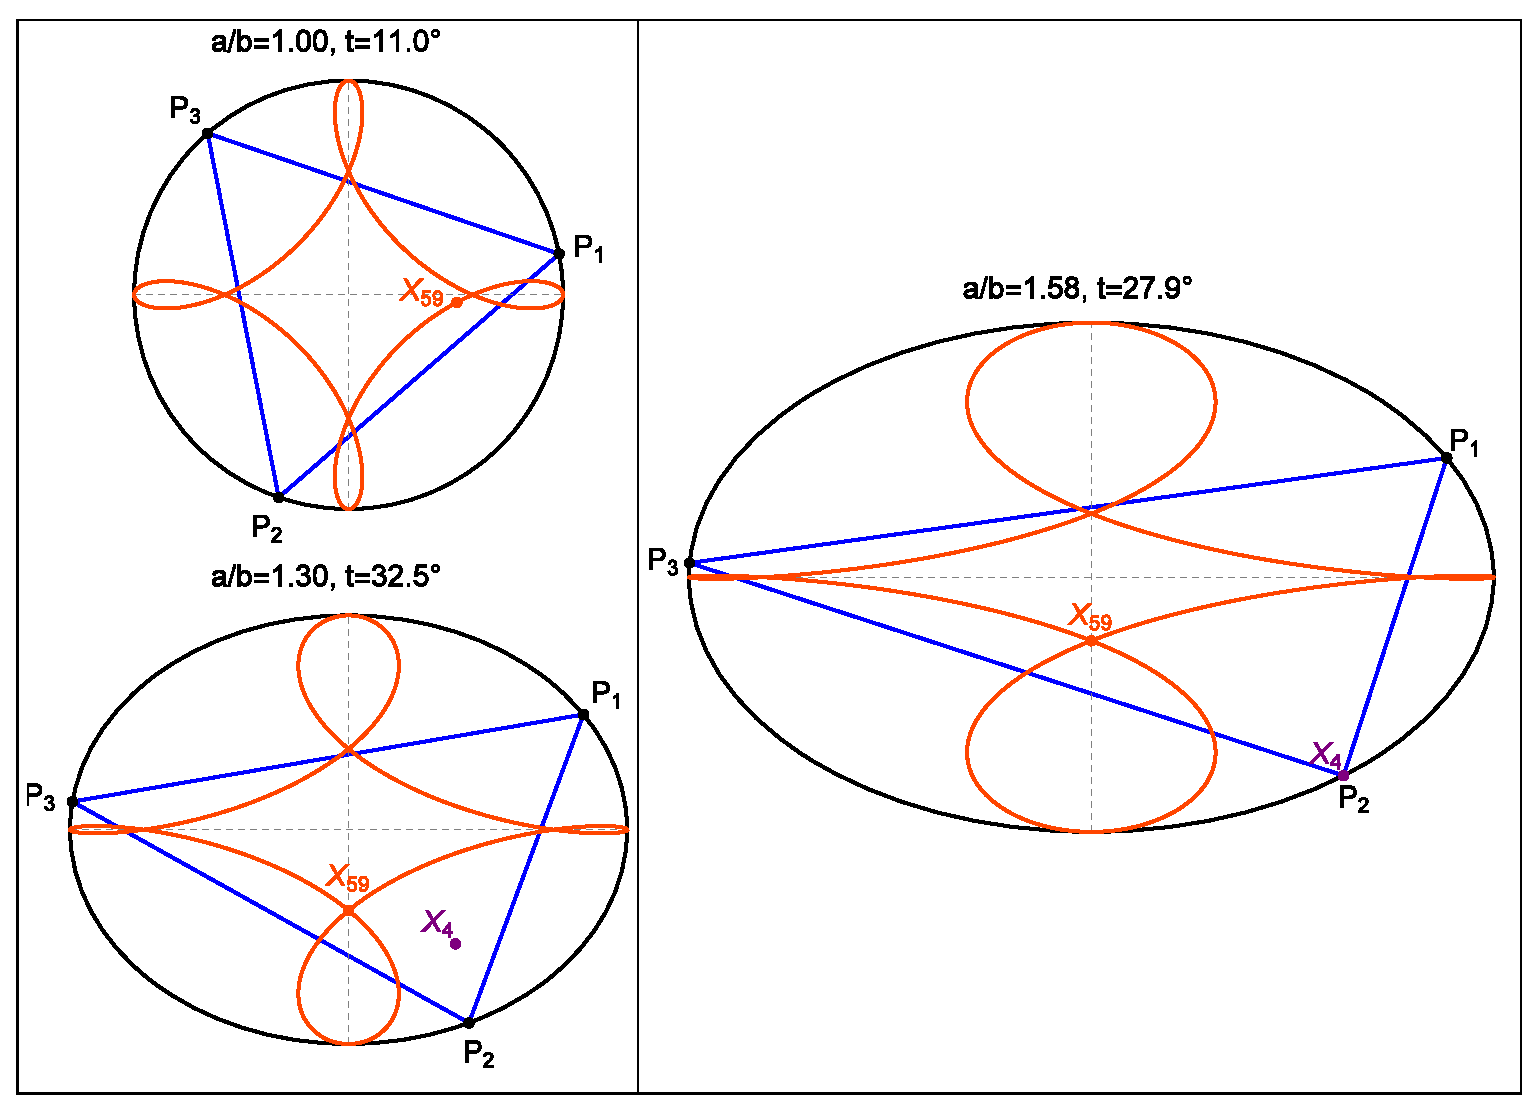
\includegraphics[width=\textwidth]{pics_04_160_x59_center.eps}
    \caption{Over billiard 3-periodics, the locus of $X_{59}$ is a continuous curve with four self-intersections, tangent to the billiard at its four vertices. \textbf{Top Left}: if $a/b$ is slightly above 1, the locus of  $X_{59}$ is nearly four-fold symmetric. Not shown: if $a/b=1$, $X_{59}$ will be on the line at infinity. \textbf{Bottom Left}: An acute 3 periodic $a/b<\alpha_4$, and an acute 3-periodic. \textbf{Right}: a right-angle 3-periodic in an $a/b>\alpha_4$ elliptic billiard. \href{https://youtu.be/pl_PqSuhlx0}{Video}, \href{https://bit.ly/3fvDlZd}{Live}}
    \label{fig:04-x59-locus}
\end{figure}

%%% end self-inter

%%% begin non-compact

%%% end non-compact

%%% EXERCISES
%%% BEGIN EXERCISES
\section{Exercises}

\begin{exercise}
Calculate the elliptic billiard aspect ratio $a/b$ such that top and bottom vertices of the elliptic locus of $X_3$ coincide each with the billiard top and bottom vertices. Repeat for the locus of $X_5$.
\end{exercise}

\begin{exercise}
Calculate the elliptic billiard aspect ration $a/b$ such that the locus of $X_4$ is identical to a $90^\circ$ rotated copy of billiard.
\end{exercise}

\begin{exercise}
Over billiard 3-periodics, the envelope of the Euler line is an astroidal-like curve with four cusps, see it \href{https://bit.ly/3yiCvrn}{Live}. Derive its equation. Also, find the elliptic billiard aspect ratio $a/b$ such that the top and bottom cusps of said curve coincide each with top and bottom vertices of the elliptic billiard.
\end{exercise}